\chapter{Arbeitsgrundlagen}
% ==================================================================
\setcounter{page}{1} \thispagestyle{fancy} 
% ==================================================================
In diesem Kapitel werden die Grundlagen zum Versuch beschrieben. Dazu gehören die theoretischen Grundlagen sowie die benötigten Formeln.

\section{Theoretische Grundlagen}
Beugung nennt man die Abweichungen von der geradlinigen Wellenausbreitung, wie sie mit Hilfe von Strahlen beschrieben wird. Diese tritt auf, wenn Wellen auf Oberflächen treffen, bei welchen sie begrenzt werden, wie z.B. Kanten oder Öffnungen\cite{Angaben2011}.\\[0.5cm]Mit Hilfe des Huygens-Fresnel’schen Prinzips können die Beugungseffekte erklärt werden: Alle Punkte hinter einer Öffnung senden Sekundär-Kugelwellen aus, deren Überlagerung das neue Wellenfeld liefert. Durch Interferenz der Kugelwellen ergibt sich so mit der Fresnel'schen oder der Frauenhofer'schen Beobachtungsart ein Muster aus Licht und Schatten an einem Schirm, das sogenannte Interferenzmuster \cite{Angaben2011}.\\

\subsection{Fresnel'sche Beobachtungsart}
Bei dieser Beobachtungsart wird ein Schirm in das Nahfeld gebracht, um das Interferenzmuster direkt beobachten zu können. Mithilfe einer Linse kann dieses Muster auf einen weiter entfernteren Schirm abgebildet werden. Das Muster auf dem weiter entfernteren Schirm ist dann jedoch von der Lage der Linse abhängig. Anordnung gemäss Abbildung \ref{fig:Fresnel} \cite{Angaben2011}.\\
%ABBILDUNG1
\begin{figure}[h]
\begin{center}
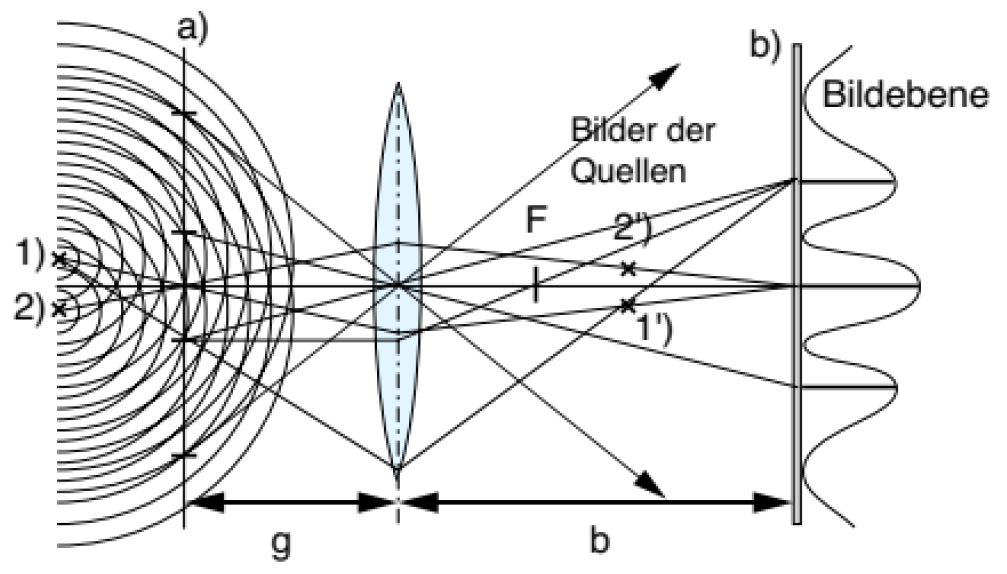
\includegraphics[scale=0.8]{Bilder/Fresnel.png} 
\end{center}
\caption[Anordnung der Fresnel'schen Beobachtungsart]{Anordnung der Fresnel'schen Beobachtungsart. Die Wellen der Quellen (1, 2) treffen auf ein Objekt mit Öffnungen im Nahfeld (a). Die Kugelwellen interferieren, wobei über eine Linse das so entstehende Interferenzmuster an einen Schirm (b) gegeben wird \cite{Angaben2011}.}
\label{fig:Fresnel}
\end{figure}

\newpage
\subsection{Frauenhofer'sche Beobachtungsart}
Bei dieser Beobachtungsart wird ein Schirm in die Brennebene einer Linse gebracht, welches das Interferenzmuster darauf abbildet. Das Interferenzmuster ist hier nicht von der Lage der Linse zur Quelle abhängig und ist bis auf einen Skalierungsfaktor identisch. Der Aufbau dieser Anordnung ist in Abbildung \ref{fig:Frauenhofer} erkennbar \cite{Angaben2011}.\\
%ABBILDUNG2
\begin{figure}[h]
\begin{center}
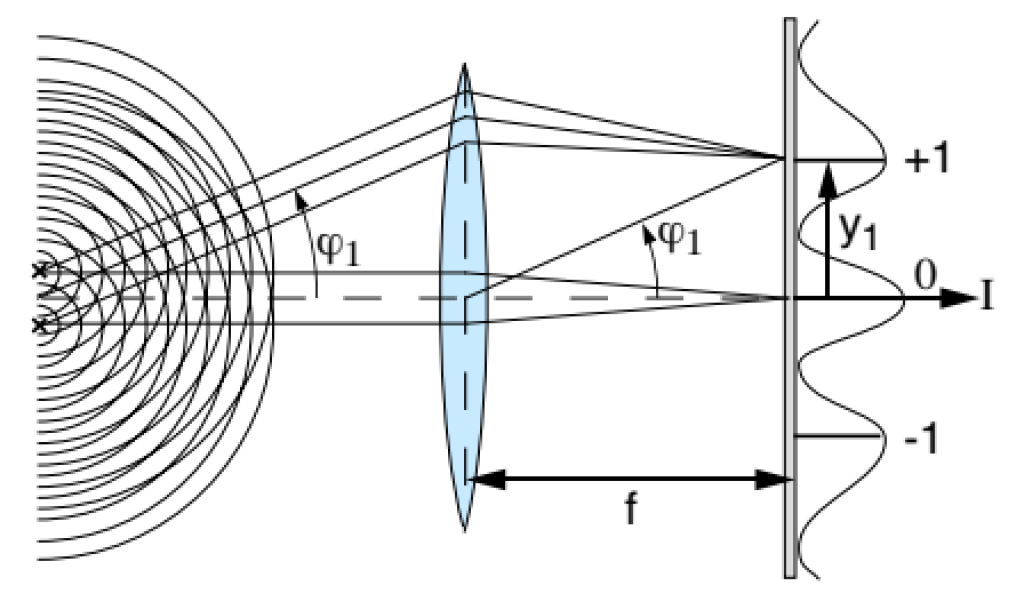
\includegraphics[scale=0.8]{Bilder/Frauenhofer.png}
\end{center}
\caption[Anordnung der Frauenhofer'schen Beobachtungsart]{Anordnung der Frauenhofer'schen Beobachtungsart. Das Interferenzmuster der Interferierenden Wellen (links) wird über eine Linse im Fernfeld auf ein Schirm gegeben. Der Schirm steht in der Brennebene (Brennweite f) der Linse. Das Interferenzmuster ist so nicht mehr Abhängig von der Linsenposition gegenüber dem Objekt \cite{Angaben2011}.}
\label{fig:Frauenhofer}
\end{figure}

\subsection{Beugung am Spalt und Antispalt}
Beugung am Einzelspalt erzeugt im Fernfeld ein Interferenzmuster, bei welchem sich helle und dunkle Bereiche abwechseln. Die hellen Bereiche sind in der Mitte am hellsten und nach aussen gehend nimmt die Intensität ab. In der Mitte ist der hellste Bereich beim Spalt bzw. der dunkelste Bereich beim Antispalt, da hier ungebeugte Strahlen direkt auftreffen bzw. gar nicht \cite{Angaben2011}.\\

\subsection{Beugung am Loch}
Bei einer Lochblende beobachtet man als Interferenzmuster konzentrisch angelegte Ringe, Maxima und Minima abwechselnd, auf dem Schirm \cite{Angaben2011}.\\
 
\subsection{Beugung am Strichgitter}
Das Interferenzmuster bei der Beugung am Strichgitter ergibt ein Interferenzmuster, bei dem entlang der Horizontalen Lichtpunkte auftreten. Diese Lichtpunkte entstehen, wie schon erwähnt, durch konstruktive Interferenz an diesen Stellen \cite{Angaben2011}.\\

\section{Benötigte Formeln}
Für die Beugung der Frauenhofer’sche Beobachtungsart gilt folgende Formel \ref{eq:1} \cite{Angaben2011}.\\
%FORMEL1 
\begin{equation}
a_{m}=f\cdot\tan\left( \arcsin\left[ \frac{m\cdot\lambda}{d}\right] \right) 
\label{eq:1}
\end{equation}
Formel \ref{eq:1} beschreibt, dass die Distanz des Maximums zur Mitte des Interferenzmusters (a$_{m}$) gleich der Brennweite (f) multipliziert mit dem Tangens ($\tan$) des Arkussinus ($\arcsin$) von der Ordnungszahl desselben Maximums (m) multipliziert mit der Wellenlänge des Lichts ($\lambda$) geteilt durch die Gitterkonstante (d) ist.\\[0.5cm]Bei der direkten Beobachtung des Interferenzmusters im Fernfeld (ohne Linse) gilt dieselbe Formel \ref{eq:1}, jedoch ist die Brennweite mit der Distanz von Objekt zum Schirm zu ersetzen.\\[0.5cm]Für die Auswertung bei der Beugung am Loch muss die Ordnungszahl der obigen Formel \ref{eq:1} angepasst werden, da es sich hier um Kreise handelt. Die neue Konstante, welche sich anstelle der Ordnungszahl einfügt, lässt sich gemäss folgende Formel \ref{eq:2} berechnen:
%FORMEL2
\begin{equation}
m_{i}=\frac{J_{1,i}}{\pi}
\label{eq:2}
\end{equation}
Formel \ref{eq:2} zeigt, dass die neue Konstante (m$_{i}$) der i-ten Nullstelle der 2. Besselfunktion (J$_{1}$) geteilt durch die Kreiszahl ($\pi$) entspricht.

\subsection{Kreiskoeffizienten für Beugung am Loch}
Die ersten 9 Konstanten (m$_{i}$), die für die Auswertung gebraucht werden, wurden gemäss Formel \ref{eq:2} berechnet und lauten wie folgt:\\

\begin{tabular}[h]{ccc}
Koeffizientennummer & J$_{1,i}$ & m$_{i}$ \\ 
\hline 
1 & 3.832 & 1.220 \\  
2 & 7.016 & 2.233 \\  
3 & 10.173 & 3.238 \\ 
4 & 13.324 & 4.241 \\ 
5 & 16.471 & 5.243 \\ 
6 & 19.616 & 6.244 \\  
7 & 22.760 & 7.245 \\ 
8 & 25.904 & 8.245 \\ 
9 & 29.047 & 9.246 \\ 
\label{table:Koeff}
\end{tabular} 
